\chapter{Organisatie van zenuwstelsels}\label{ch:b3:nervous-systems}

Een kwal heeft enkele duizenden neuronen in een net zonder centrum en
kan zwemmen, eten en zich oprichten. Een octopus heeft er een half
miljard, twee derde daarvan in zijn armen, die elk een probleem kunnen
oplossen waarvan het brein niets te horen heeft gekregen. De mens heeft
er zesentachtig miljard, verbonden door honderd biljoen synapsen,
draaiend op twintig watt --- een vijfde van zijn energie voor twee
procent van zijn massa --- en Santiago Ramón y Cajal, die ze in de
jaren 1890 cel voor cel tekende naar met zilver gekleurde coupes, zag
dat het afzonderlijke cellen waren die elkaar raakten zonder te
versmelten en dat de signalen er in één richting doorheen liepen. Het
vorige deel behandelde het neuron: zijn rustpotentiaal, zijn
actiepotentiaal, zijn synaps. Dit hoofdstuk behandelt waarin neuronen
zijn ingebouwd: de passieve kabel die bepaalt hoe ver een signaal zich
uitbreidt en hoe snel, de schakelingen --- reflex, oscillator, remmende
omgeving --- waaruit gedrag wordt samengesteld, de bouw van het
zenuwstelsel van de gewervelden en van de \omterm{def:b3:nervous-systems:cells}{glia} die het draaiende
houden, zijn energiebegroting, en de manieren waarop verschillende
dieren hun neuronen hebben verdeeld.

\section{Neuronen en glia}

\begin{definition}[De cellen van het zenuwstelsel]\label{def:b3:nervous-systems:cells}
\index{neuron!typen}\index{glia}\index{astrocyt}\index{oligodendrocyt}\index{myeline}\index{microglia}\index{interneuron}
Neuronen komen in een handvol bouwvormen voor die overal in het brein
terugkeren: \emph{piramidale} cellen, de excitatoire projectieneuronen
van de schors, met een lange apicale dendriet en een axon dat een meter
kan afleggen; \emph{Purkinje}-cellen van de \omterm{def:b3:nervous-systems:plan}{kleine hersenen}, wier platte
dendrietenboom tweehonderdduizend synapsen ontvangt; sensorische
neuronen met één uitloper naar de periferie en één naar het merg; en
\emph{interneuronen}, cellen met een kort axon die binnen één gebied
blijven, de meeste ervan remmend. Ongeveer vier op de vijf neuronen van
de schors geven glutamaat af en prikkelen; één op de vijf geeft GABA af
en remt. De \emph{glia}, even talrijk als de neuronen, doen de rest.
\emph{Astrocyten} omwikkelen synapsen en bloedvaten: zij nemen het
kalium op dat vurende neuronen afgeven en het glutamaat dat synapsen
morsen, leveren lactaat, regelen plaatselijk de doorbloeding, en wekken
de bloed--hersenbarrière op en houden haar in stand.
\emph{Oligodendrocyten} in het centrale zenuwstelsel en
\emph{Schwann-cellen} in de periferie omwikkelen axonen met
\emph{myeline}, tientallen lagen membraan die het axon isoleren tussen
de knopen waar de kanalen zitten. \emph{Microglia} zijn de vaste
\omterm{def:b3:innate-immunity:innate}{macrofagen} van het brein: zij snoeien synapsen tijdens de ontwikkeling
en ruimen puin op. Ependymcellen bekleden de ventrikels en maken het
\omterm{prop:b3:nervous-systems:barrier-budget}{hersenvocht}.
\end{definition}

\begin{proof}[Bewijsmateriaal]
De zilverchromaatkleuring van Golgi (1873) zwartte om redenen die
onbekend zijn ongeveer één neuron op honderd volledig en liet de rest
onzichtbaar ---
zodat één cel in haar geheel zichtbaar werd in een kluwen van
miljoenen. Golgi las zijn eigen preparaten als een doorlopend netwerk;
Cajal zag vanaf 1888, met dezelfde kleuring op embryonaal weefsel waar
de cellen eenvoudiger zijn, dat elke cel vrij eindigde, dat dendrieten
en axon verschilden, en dat axonen eindigden op de dendrieten en de
lichamen van andere cellen zonder zich ermee te verbinden. Uit de
rangschikking van sensorische en motorische cellen leidde hij de
richting van de stroom af --- dendriet naar lichaam naar axon --- de
\emph{wet van de dynamische polarisatie}. Sherrington noemde de spleet
in 1897 de \emph{synaps}; de elektronenmicroscoop liet haar in 1954
zien.
\end{proof}

\begin{omfigure}
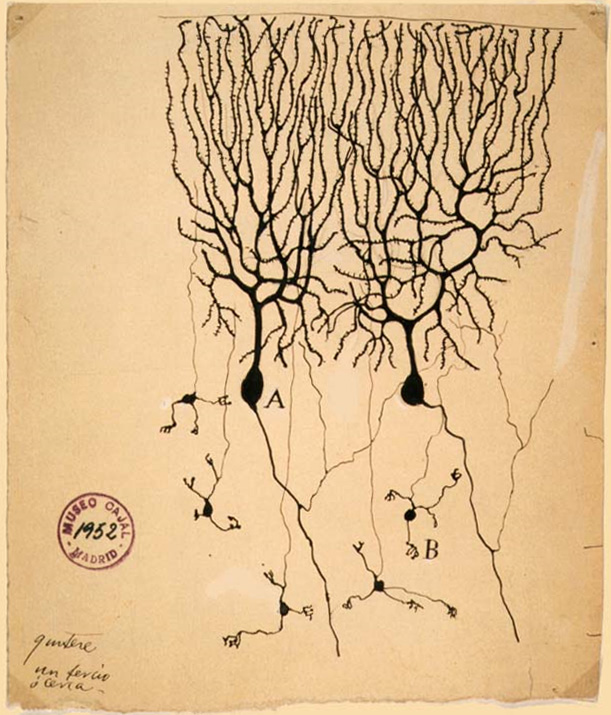
\includegraphics[width=0.30\linewidth]{images/book5/cajal-purkinje.jpg}\hspace{0.04\linewidth}
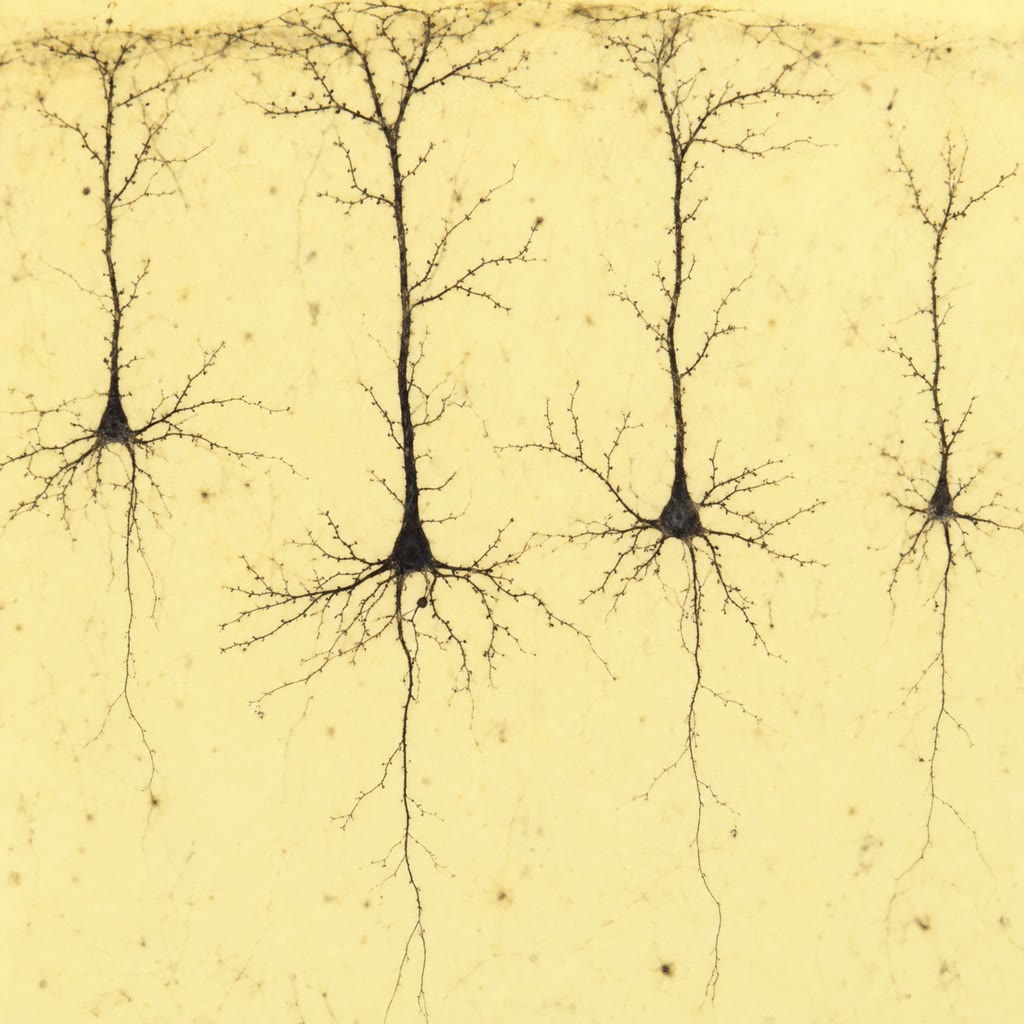
\includegraphics[width=0.30\linewidth]{images/book5/ai/b5-17-cortex-neurons.jpg}\hspace{0.04\linewidth}
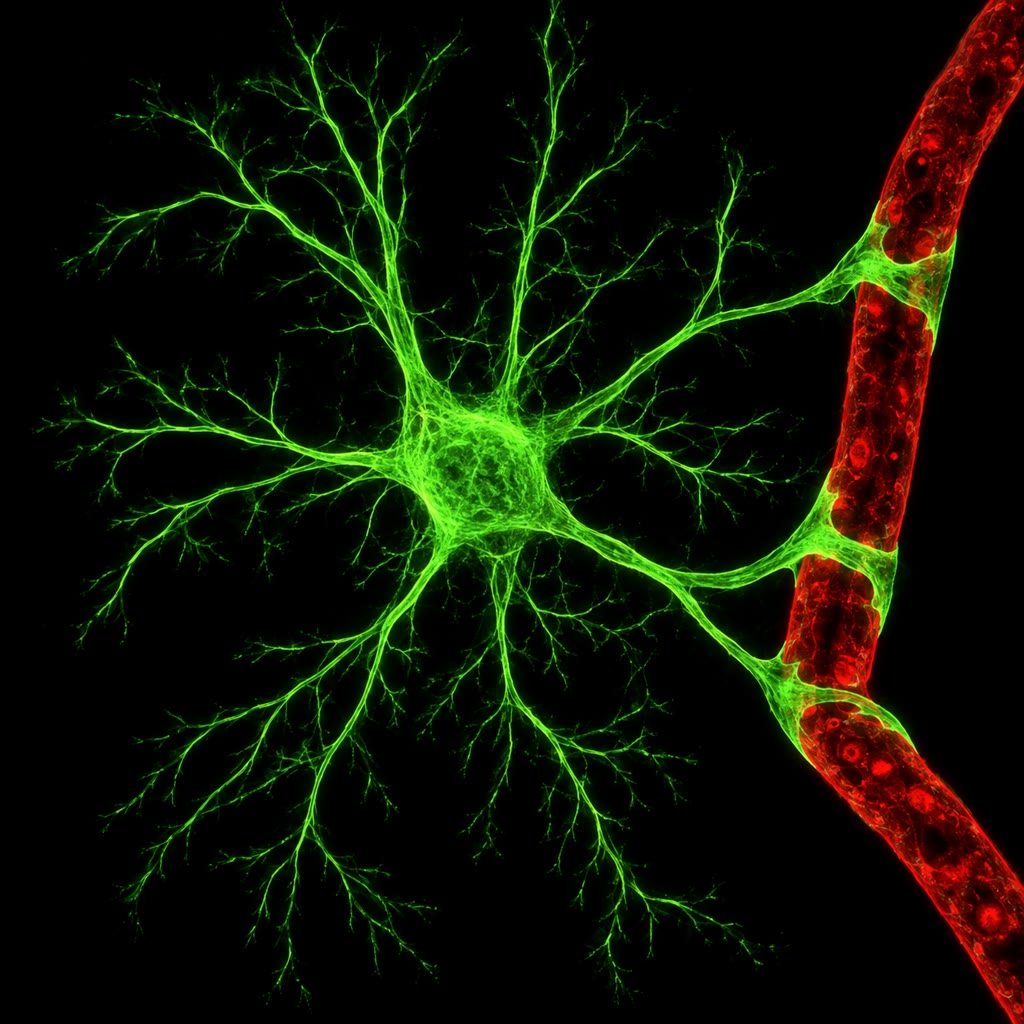
\includegraphics[width=0.30\linewidth]{images/book5/ai/b5-17-astrocyte.jpg}

{\small Links: een Purkinje-cel van de \omterm{def:b3:nervous-systems:plan}{kleine hersenen}, getekend door
Cajal (1899) naar een met Golgi gekleurde coupe --- de hele
dendrietenboom van één cel, het argument voor het neuron als eenheid
(publiek domein). Midden: piramidale neuronen van de schors in een
Golgi-kleuring. Rechts: een \omterm{def:b3:nervous-systems:cells}{astrocyt} (groen) met zijn eindvoetjes op een
haarvat (rood).}
\end{omfigure}

\section{Het neuron als kabel}

\begin{theorem}[De kabelvergelijking in de stationaire toestand]\label{thm:b3:nervous-systems:cable}
\index{kabelvergelijking}\index{lengteconstante}\index{tijdconstante!membraan}\index{geleidingssnelheid}
Beschouw een dendriet of een ongemyeliniseerd axon als een cilinder met
diameter $d$, waarvan het cytoplasma soortelijke weerstand $R_{i}$
heeft en het membraan een specifieke weerstand $R_{m}$ (weerstand maal
oppervlak) en een capaciteit $C_{m}$ per oppervlak. Per lengte-eenheid
is de axiale weerstand $r_{i} = 4R_{i}/\pi d^{2}$
en de membraanweerstand $r_{m} = R_{m}/\pi d$. Een gelijkblijvende
spanning $V_{0}$ die bij $x = 0$ wordt aangelegd, breidt zich langs de
vezel uit als
\[
V(x) = V_{0}\,e^{-x/\lambda}, \qquad
\lambda = \sqrt{\frac{r_{m}}{r_{i}}} = \sqrt{\frac{R_{m}\,d}{4R_{i}}},
\]
waarin $\lambda$ de \emph{\omterm{thm:b3:nervous-systems:cable}{lengteconstante}} is: de afstand waarover een
passief signaal tot $1/e$ daalt, toenemend met de wortel uit de
diameter. Het membraan laadt op met de \emph{tijdconstante} $\tau =
R_{m}C_{m}$, onafhankelijk van de meetkunde. Een actiepotentiaal, die
zichzelf hernieuwt, loopt langs een ongemyeliniseerd axon met een
snelheid evenredig met $\lambda/\tau$ en dus met $\sqrt{d}$; langs een
gemyeliniseerd axon, waar hij van knoop naar knoop springt, met een
snelheid evenredig met $d$ --- ongeveer \qty{6}{m/s} per micrometer
diameter.
\end{theorem}
\begin{proof}
Zij $I(x)$ de axiale stroom. De wet van Ohm langs de kern geeft
$\mathrm{d}V/\mathrm{d}x = -r_{i}I$; behoud van lading in de
stationaire toestand zegt dat de axiale stroom die tussen $x$ en $x + \mathrm{d}x$
verloren gaat door het membraan lekt, $\mathrm{d}I/\mathrm{d}x = -V/r_{m}$.
Door de eerste te differentiëren en de tweede in te vullen ontstaat
$\mathrm{d}^{2}V/\mathrm{d}x^{2} = (r_{i}/r_{m})V = V/\lambda^{2}$, een
lineaire tweede-ordevergelijking waarvan de oplossing die begrensd blijft als $x \to \infty$ luidt
$V_{0}e^{-x/\lambda}$. Invullen van $r_{m} = R_{m}/\pi d$ en $r_{i} =
4R_{i}/\pi d^{2}$ geeft $\lambda^{2} = R_{m}d/4R_{i}$. De tijdconstante
is die van een weerstand en een condensator parallel, $r_{m}c_{m} =
(R_{m}/\pi d)(C_{m}\pi d) = R_{m}C_{m}$. Voor de snelheden: een
hernieuwende golf moet het membraan een \omterm{thm:b3:nervous-systems:cable}{lengteconstante} vooruit opladen
in ongeveer een tijdconstante, dus $v \sim \lambda/\tau \propto \sqrt{d}$;
tussen de knopen van een gemyeliniseerd axon heeft het membraan een
weerstand die is verhoogd en een capaciteit die is verlaagd door de ruim
honderd lagen \omterm{def:b3:nervous-systems:cells}{myeline}, schaalt de afstand tussen de knopen met $d$, en is het resultaat
$v \propto d$. De evenredigheidsconstanten worden aangenomen.
\end{proof}

\begin{example}[Getallen voor een dendriet en twee axonen]\label{ex:b3:nervous-systems:numbers}
Een dendriet met $d = \qty{2}{\micro m}$, $R_{m} = \qty{2e4}{\ohm.cm^2}$
en $R_{i} = \qty{100}{\ohm.cm}$: $\lambda = \sqrt{2\times 10^{4}\times
2\times 10^{-4}/400}\ \unit{cm} = \qty{0.1}{cm} = \qty{1}{mm}$ --- een
synaptische potentiaal aan de punt van een dendriet van een millimeter
bereikt het cellichaam met een derde van haar grootte, en daarom maakt
de meetkunde van een dendrietenboom deel uit van zijn berekening.
$\tau = 2\times 10^{4}\times
10^{-6}\,\unit{F/cm^2}\cdot\unit{\ohm.cm^2} = \qty{20}{ms}$, het venster
waarbinnen invoeren moeten aankomen om op te tellen. Het reuzenaxon van
een inktvis van \qty{500}{\micro m}, ongemyeliniseerd, geleidt met
ongeveer \qty{25}{m/s}; om hetzelfde te bereiken gebruikt een gewervelde
een gemyeliniseerd axon van \qty{4}{\micro m}, in doorsnede
vijftienduizend maal kleiner --- de reden dat een zenuw van een
gewervelde tienduizend snelle vezels kan dragen in de ruimte van één
inktvisaxon. Een motorisch axon van \qty{20}{\micro m} geleidt met
\qty{120}{m/s}; strijkt multiple sclerose zijn \omterm{def:b3:nervous-systems:cells}{myeline} weg, dan daalt de
snelheid tienvoudig en kan de geleiding op de kale stukken geheel
uitvallen.
\end{example}

\begin{omfigure}
\begin{tikzpicture}
\begin{axis}[
  width=6.4cm, height=5.2cm,
  axis x line=bottom, axis y line=left,
  xmin=0, xmax=3, ymin=0, ymax=1.05,
  xlabel={afstand (mm)}, ylabel={$V/V_{0}$},
  xlabel style={font=\small, at={(axis description cs:0.5,-0.12)}, anchor=north}, ylabel style={font=\small},
  tick label style={font=\scriptsize}, xtick={0,1,2,3}, ytick={0,0.37,1}, yticklabels={0,$1/e$,1},
  clip=false,
]
\addplot[very thick, omDef, domain=0:3, samples=60] {exp(-x/1.0)};
\addplot[very thick, omThm, domain=0:3, samples=60] {exp(-x/0.5)};
\node[font=\scriptsize, omDef, anchor=south west] at (axis cs:1.2,0.45) {$d = \qty{2}{\micro m}$, $\lambda = \qty{1}{mm}$};
\node[font=\scriptsize, omThm, anchor=north west] at (axis cs:0.8,0.22) {$d = \qty{0.5}{\micro m}$, $\lambda = \qty{0.5}{mm}$};
\end{axis}
\begin{axis}[
  at={(7.6cm,0)}, anchor=south west,
  width=6.4cm, height=5.2cm,
  xmode=log, ymode=log,
  xmin=0.1, xmax=1000, ymin=0.1, ymax=200,
  xlabel={axondiameter ($\unit{\micro m}$)}, ylabel={snelheid (m/s)},
  xlabel style={font=\small, at={(axis description cs:0.5,-0.12)}, anchor=north}, ylabel style={font=\small},
  tick label style={font=\scriptsize},
  clip=false,
]
\addplot[very thick, omDef, domain=1:25, samples=2] {6*x};
\addplot[very thick, omThm, domain=0.2:1000, samples=2] {1.1*sqrt(x)};
\fill[omThm] (axis cs:500,25) circle (2pt); \node[font=\scriptsize, anchor=north east] at (axis cs:500,23) {reuzenaxon van de inktvis};
\fill[omDef] (axis cs:20,120) circle (2pt); \node[font=\scriptsize, anchor=west] at (axis cs:26,120) {motorisch axon van de mens};
\node[font=\scriptsize, omDef, anchor=north west, align=left] at (axis cs:1.2,60) {gemyeliniseerd: $v \propto d$};
\node[font=\scriptsize, omThm, anchor=north west, align=left] at (axis cs:2,0.7) {ongemyeliniseerd: $v \propto \sqrt{d}$};
\end{axis}
\end{tikzpicture}

{\small Links: het passieve verval van een gelijkblijvend signaal langs
een dendriet, voor twee diameters --- de \omterm{thm:b3:nervous-systems:cable}{lengteconstante} groeit als
$\sqrt{d}$. Rechts: geleidingssnelheid tegen diameter; \omterm{def:b3:nervous-systems:cells}{myeline} laat een
vezel van \qty{4}{\micro m} doen waarvoor een ongemyeliniseerd axon een
halve millimeter nodig heeft.}
\end{omfigure}

\section{Schakelingen}

\begin{definition}[Elementaire schakelingen]\label{def:b3:nervous-systems:circuits}
\index{reflexboog}\index{wederzijdse remming}\index{voorwaartse remming}\index{terugkoppelingsremming}\index{convergentie}\index{divergentie}
Een \emph{reflexboog} is de kortste weg van een zintuig naar een
uitvoerend orgaan: bij de kniepeesreflex komt een afferente vezel uit
een spierspoel het merg binnen en schakelt rechtstreeks over op de
motorneuronen van dezelfde spier, die haar ongeveer \qty{30}{ms} na de
tik samentrekken --- één synaps, geen brein. Diezelfde afferente vezel
prikkelt een remmend \omterm{def:b3:nervous-systems:cells}{interneuron} naar de motorneuronen van de
tegenwerkende spier (\emph{wederzijdse remming}), zodat de
samentrekking van de strekker niet door de buiger wordt bestreden. De
meeste schakelingen zijn uit enkele motieven opgebouwd:
\emph{divergentie}, één neuron dat er vele aanstuurt, en
\emph{convergentie}, vele op één, wat aanwijzingen optelt;
\emph{voorwaartse remming}, waarbij een invoer zowel een doelcel
prikkelt als een \omterm{def:b3:nervous-systems:cells}{interneuron} dat de doelcel een milliseconde later
remt, wat het antwoord in de tijd scherpt;
\emph{terugkoppelingsremming}, waarbij de uitvoer van de doelcel zelf
een \omterm{def:b3:nervous-systems:cells}{interneuron} prikkelt dat haar remt, wat het vuren begrenst en, naar
de buren uitgebreid, de laterale remming voortbrengt die het contrast
scherpt (\cref{ch:b3:sensory-systems}); en \emph{ontremming}, het
remmen van een remmer, de manier waarop de basale kernen een beweging
vrijgeven.
\end{definition}

\begin{omfigure}
\begin{tikzpicture}[every node/.style={font=\scriptsize}, >=stealth]
  % spinal cord cross-section (schematic)
  \draw[thick, omDef!60, fill=omDef!8] (5.4,1.5) ellipse (2.0 and 1.5);
  \draw[thick, gray, fill=gray!15] (5.4,1.5) .. controls (4.7,2.4) and (4.0,2.6) .. (4.0,1.9) .. controls (4.0,1.2) and (4.6,0.9) .. (4.8,0.5) .. controls (5.0,0.2) and (5.8,0.2) .. (6.0,0.5) .. controls (6.2,0.9) and (6.8,1.2) .. (6.8,1.9) .. controls (6.8,2.6) and (6.1,2.4) .. (5.4,1.5);
  \node[above] at (5.4,3.05) {ruggenmerg};
  % muscles
  \draw[thick, omMeth!70!black, fill=omMeth!20] (0.2,0.2) rectangle (1.4,2.0); \node[below, align=center] at (0.8,0.1) {strekker\\(quadriceps)};
  \draw[thick, omThm!70!black, fill=omThm!15] (0.2,-2.6) rectangle (1.4,-1.4); \node[below, align=center] at (0.8,-2.7) {buiger\\(hamstring)};
  \fill[omProp] (0.8,1.3) ellipse (0.12 and 0.3); \node[left, font=\tiny] at (0.65,1.3) {spierspoel};
  % Ia afferent to cord (dorsal)
  \draw[very thick, omProp] (0.9,1.3) .. controls (2.0,2.6) and (3.6,2.9) .. (4.8,2.2); \fill[omProp] (4.8,2.2) circle (0.09);
  \node[above, omProp] at (2.6,2.85) {Ia-afferent: rek};
  % motor neuron to extensor
  \fill[omMeth!70!black] (5.0,0.9) circle (0.16);
  \draw[->, very thick, omMeth!70!black] (4.9,0.85) .. controls (3.4,0.3) and (2.0,0.4) .. (1.4,1.0);
  \draw[->, thick, omProp] (4.8,2.2) -- (5.0,1.1);
  % inhibitory interneuron to flexor motor neuron
  \fill[omThm] (6.1,1.7) circle (0.13);
  \draw[->, thick, omProp] (4.9,2.25) -- (6.0,1.8);
  \fill[omThm!70!black] (6.0,0.6) circle (0.16);
  \draw[-|, thick, omThm] (6.1,1.55) -- (6.0,0.8);
  \draw[->, very thick, omThm!70!black, dashed] (5.9,0.5) .. controls (4.8,-0.8) and (3.0,-1.6) .. (1.4,-2.0);
  % right-hand labels with leaders
  \node[right, omThm, font=\tiny] at (7.6,1.9) {remmend Ia-interneuron}; \draw[gray, thin] (7.55,1.9) -- (6.25,1.7);
  \node[right, omMeth!70!black, font=\tiny, align=left] at (7.6,1.1) {motorneuron strekker: geprikkeld}; \draw[gray, thin] (7.55,1.1) -- (5.15,0.9);
  \node[right, omThm!70!black, font=\tiny, align=left] at (7.6,0.3) {motorneuron buiger: geremd}; \draw[gray, thin] (7.55,0.3) -- (6.15,0.6);
  \node[below] at (4.6,-0.15) {monosynaptische reflex: $\sim$\qty{30}{ms}};
  \node[below, align=center] at (4.2,-2.0) {wederzijdse remming:\\de tegenspeler ontspant};
\end{tikzpicture}

{\small De rekreflex. Een tik rekt de spoelen van de strekker; de
Ia-afferent prikkelt rechtstreeks de motorneuronen van de strekker (één
synaps) en legt via een remmend \omterm{def:b3:nervous-systems:cells}{interneuron} die van de buiger stil.}
\end{omfigure}

\begin{proposition}[Centrale patroongeneratoren]\label{prop:b3:nervous-systems:cpg}
\index{centrale patroongenerator}\index{halfcentrumoscillator}
Ritmische bewegingen --- ademen, lopen, zwemmen, kauwen --- worden
voortgebracht door schakelingen in de \omterm{def:b3:nervous-systems:plan}{hersenstam} en het \omterm{def:b3:nervous-systems:plan}{ruggenmerg} die
uit zichzelf oscilleren, \emph{\omterm{prop:b3:nervous-systems:cpg}{centrale patroongeneratoren}}, die de
sensorische terugkoppeling bijstelt maar niet schept: het van het brein
losgesneden \omterm{def:b3:nervous-systems:plan}{ruggenmerg} van een kat, ook beroofd van zijn sensorische
zenuwen, brengt nog altijd het afwisselende patroon van het stappen
voort. Het eenvoudigste ontwerp is het \emph{halve centrum} van Brown
(1911): twee groepen neuronen die elkaar over en weer remmen. Welke van
beide ook vuurt, zij legt haar partner stil; maar een vurende groep
raakt vermoeid --- haar kanalen inactiveren, haar remming van de
partner verzwakt --- en de partner, bevrijd, vuurt en legt op haar
beurt de eerste stil: afwisseling, met een periode die door de
tijdconstante van de vermoeidheid wordt bepaald en niet door een klok.
Het ademhalingsritme ontstaat in een groepje van enkele duizenden
neuronen in het verlengde merg (het pre-Bötzinger-complex), dat van de
geboorte tot de dood in salvo's vuurt; het zwemmen van de prik is een
keten van halve centra langs zijn merg, elk vertraagd ten opzichte van
het vorige zodat er een golf staartwaarts loopt.
\end{proposition}

\begin{omfigure}
\begin{tikzpicture}[every node/.style={font=\scriptsize}, >=stealth]
  % half-centre
  \begin{scope}
    \draw[thick, fill=omDef!25] (0,0) circle (0.5); \node at (0,0) {L};
    \draw[thick, fill=omThm!25] (3,0) circle (0.5); \node at (3,0) {R};
    \draw[-|, very thick] (0.5,0.2) -- (2.5,0.2); \draw[-|, very thick] (2.5,-0.2) -- (0.5,-0.2);
    \node[above] at (1.5,0.3) {wederzijdse remming};
    \draw[->, thick, omDef] (0,-0.5) -- (0,-1.3) node[below] {linkerspieren};
    \draw[->, thick, omThm] (3,-0.5) -- (3,-1.3) node[below] {rechterspieren};
    \draw[->, thick, gray] (-1.2,0.6) -- (-0.45,0.25) node[pos=0, above, align=center] {tonische aandrijving\\vanuit de hersenstam};
    \draw[->, thick, gray] (4.5,0.6) -- (3.45,0.25);
  \end{scope}
  % traces
  \begin{scope}[xshift=6.0cm, yshift=0.9cm]
    \node[left, omDef] at (0,0) {L};
    \foreach \x in {0,2,4} { \foreach \s in {0.1,0.2,...,0.9} \draw[omDef] (\x+\s,-0.15) -- (\x+\s,0.15); }
    \node[left, omThm] at (0,-1.0) {R};
    \foreach \x in {1,3,5} { \foreach \s in {0.1,0.2,...,0.9} \draw[omThm] (\x+\s,-1.15) -- (\x+\s,-0.85); }
    \draw[->] (0,-1.6) -- (6.2,-1.6) node[right] {tijd};
    \draw[<->] (0,-2.0) -- (2,-2.0) node[midway, below] {periode: bepaald door de vermoeidheid};
  \end{scope}
\end{tikzpicture}

{\small Een halfcentrumoscillator. Twee groepen die elkaar remmen
wisselen elkaar onder een gelijkblijvende aandrijving af: de actieve
kant raakt vermoeid, haar remming verzwakt, de andere kant ontsnapt en
neemt het over. Geen enkel neuron is zelf ritmisch.}
\end{omfigure}

\begin{method}[Een schakeling in kaart brengen]\label{met:b3:nervous-systems:tracing}
\index{schakeling in kaart brengen}\index{optogenetica}
Om vast te stellen dat neuron A neuron B aanstuurt en dat die weg van
belang is voor een gedrag: (1) anatomie --- spuit een merkstof in die
langs axonen reist (een kleurstof, een gewijzigd rabiësvirus dat één
synaps achterwaarts oversteekt) en zoek de verbonden cellen;
(2) fysiologie --- meet aan B terwijl A wordt geprikkeld, en bepaal de
latentie (een monosynaptische verbinding geeft een vaste vertraging van
ongeveer een milliseconde) en het teken (prikkeling of remming);
(3) noodzaak --- leg A stil, door een laesie, door koeling, of door er
een lichtgestuurde chloridepomp in tot expressie te brengen en licht te
geven (\emph{optogenetica}), en kijk of het gedrag uitvalt;
(4) toereikendheid --- activeer alleen A, met een lichtgestuurd
kationkanaal, en kijk of het gedrag verschijnt; (5) breng in een intact
dier met een calciumindicator de activiteit van de hele populatie in
beeld terwijl het gedrag wordt uitgevoerd. Een schakeling staat vast
wanneer alle vijf het eens zijn; de meeste gepubliceerde schakelingen
hebben er twee of drie.
\end{method}

\section{De bouw van het zenuwstelsel van de gewervelden}

\begin{definition}[Centrale en perifere delen]\label{def:b3:nervous-systems:plan}
\index{ruggenmerg}\index{hersenstam}\index{kleine hersenen}\index{thalamus}\index{hypothalamus}\index{hersenschors}\index{autonoom zenuwstelsel}\index{enterisch zenuwstelsel}
Het \emph{centrale zenuwstelsel} is het brein en het ruggenmerg; het
\emph{perifere} is al het overige. Het \emph{ruggenmerg} ontvangt
sensorische axonen door zijn achterwortels en zendt motorische axonen
door zijn voorwortels; zijn grijze stof is een vlinder van
cellichamen, zijn witte stof zijn de gemyeliniseerde banen die op en
neer lopen. De \emph{hersenstam} --- verlengde merg, brug,
middenhersenen --- bevat de kernen van de hersenzenuwen en de centra
die ademhaling, hartslag en bloeddruk zonder nadenken gaande houden;
hersenstamdood is de dood. De \emph{kleine hersenen}, met meer neuronen
dan de rest van het brein, stemmen de tijdsordening en de coördinatie
van beweging af en leren uit de fout. De \emph{thalamus} geeft elk
zintuig behalve de reuk door aan de schors en de antwoorden van de
schors weer terug; de \emph{hypothalamus} daaronder voert de
homeostase --- temperatuur, honger, dorst, de klok, de hormoonassen van
\cref{ch:b3:endocrinology}. De \emph{basale kernen} kiezen tussen
mogelijke handelingen; de \emph{hippocampus} maakt herinneringen
(\cref{ch:b3:learning-memory}); en de \emph{hersenschors}, een blad van
zes lagen cellen, twee tot vier millimeter dik en een kwart vierkante
meter groot, gevouwen om te passen, doet de rest, in gebieden die voor
elk zintuig en elke beweging in kaart zijn gebracht en in
associatiegebieden daartussen. Het \emph{autonome} deel van het
perifere stelsel bestuurt de organen: de \emph{sympathische} keten, die
noradrenaline afgeeft, mobiliseert (hart omhoog, darm omlaag, pupillen
wijd); de \emph{parasympathische} zenuwen, die acetylcholine afgeven,
sparen en verteren; en het \emph{enterische} zenuwstelsel, een half
miljard neuronen in de darmwand, voert de spijsvertering geheel
zelfstandig uit.
\end{definition}

\begin{omfigure}
\begin{tikzpicture}[every node/.style={font=\scriptsize}, >=stealth]
  % sagittal brain schematic
  \draw[thick, omDef!70, fill=omDef!15] (0,2.0) .. controls (0,4.6) and (3.5,5.4) .. (6.0,4.4) .. controls (7.6,3.7) and (7.4,2.2) .. (6.2,1.9) .. controls (5.4,1.7) and (5.2,1.3) .. (4.4,1.6) .. controls (3.0,1.3) and (1.2,1.4) .. (0,2.0);
  \node[align=center] at (3.0,3.9) {hersenschors: zes lagen,\\sensorische, motorische en associatiegebieden};
  % basal ganglia / hippocampus (deep)
  \draw[thick, omProp!70, fill=omProp!25] (3.2,2.6) ellipse (0.9 and 0.45); \node[font=\tiny] at (3.2,2.6) {basale kernen};
  \draw[thick, omProp!70, fill=omProp!25] (5.2,2.45) ellipse (0.88 and 0.3); \node[font=\tiny] at (5.2,2.45) {hippocampus};
  % thalamus, hypothalamus
  \draw[thick, omMeth!70!black, fill=omMeth!25] (4.0,1.95) ellipse (0.7 and 0.3); \node[font=\tiny] at (4.0,1.95) {thalamus};
  \draw[thick, omMeth!70!black, fill=omMeth!40] (4.0,1.42) ellipse (0.78 and 0.22); \node[font=\tiny] at (4.0,1.42) {hypothalamus};
  % cerebellum
  \draw[thick, omThm!70, fill=omThm!20] (6.6,1.2) ellipse (0.9 and 0.6); \node[font=\tiny] at (6.6,1.2) {kleine hersenen};
  % brainstem
  \draw[thick, gray!70, fill=gray!20] (4.7,1.2) -- (5.5,1.2) -- (5.9,-0.3) -- (5.1,-0.3) -- cycle; \node[font=\tiny, rotate=-75] at (5.3,0.45) {hersenstam};
  % spinal cord
  \draw[thick, gray!70, fill=gray!20] (5.2,-0.3) rectangle (5.8,-1.6); \node[right, font=\tiny] at (5.85,-1.0) {ruggenmerg};
  % labels with leaders on the right
  \node[right, align=left] at (7.8,3.4) {thalamus: doorgeefluik van elk\\zintuig behalve de reuk; hypothalamus:\\homeostase, klok, hormoonassen};
  \draw[gray] (7.75,3.3) -- (4.7,1.95);
  \node[right, align=left] at (7.8,1.9) {kleine hersenen: tijdsordening en\\coördinatie, leren uit de fout};
  \draw[gray] (7.75,1.8) -- (7.5,1.4);
  \node[right, align=left] at (7.8,0.4) {hersenstam: ademhaling, hart,\\hersenzenuwen (verlengde merg,\\brug, middenhersenen)};
  \draw[gray] (7.75,0.4) -- (5.9,0.4);
  \node[right, align=left] at (7.8,-1.0) {ruggenmerg: reflexen, patroon-\\generatoren, banen op en neer};
\end{tikzpicture}

{\small Het brein van een gewervelde in aanzicht van opzij,
schematisch: de schors boven de diepe kernen, de \omterm{def:b3:nervous-systems:plan}{thalamus} en de
\omterm{def:b3:nervous-systems:plan}{hypothalamus} in het midden, de \omterm{def:b3:nervous-systems:plan}{kleine hersenen} daarachter, de \omterm{def:b3:nervous-systems:plan}{hersenstam}
die overgaat in het merg.}
\end{omfigure}

\begin{proposition}[De bloed--hersenbarrière en de begroting van het brein]\label{prop:b3:nervous-systems:barrier-budget}
\index{bloed-hersenbarrière}\index{hersenvocht}\index{energiebegroting van het brein}
De haarvaten van het brein zijn afgesloten door nauwe verbindingen
tussen hun endotheelcellen, omwikkeld met eindvoetjes van \omterm{def:b3:nervous-systems:cells}{astrocyten} en
uitgerust met transporteiwitten die glucose en aminozuren toelaten en
veel andere stoffen naar buiten pompen: de
\emph{bloed--hersenbarrière}, die de ionensamenstelling van de
extracellulaire vloeistof van het brein constant houdt omwille van het
elektrische gedrag van de neuronen, en die de meeste geneesmiddelen
buitensluit (\qty{98}{\%} van de kleine moleculen, alle antilichamen)
--- het centrale probleem van de neurofarmacologie. Het brein drijft in
\qty{150}{mL} \emph{\omterm{prop:b3:nervous-systems:barrier-budget}{hersenvocht}}, dat met een halve milliliter per
minuut wordt gemaakt en viermaal per dag wordt vernieuwd, dat het
schokken opvangt en afval afvoert, vooral tijdens de slaap. De kosten
van het brein: ongeveer \qty{20}{W} bij een volwassene, \qty{20}{\%}
van de rustverbranding, bijna alles als glucose die tot ATP wordt
verbrand, en het meeste van dat ATP wordt uitgegeven door de
natriumpomp, die de gradiënten herstelt die actiepotentialen en
synaptische stromen uitputten. Bij \qty{50}{kJ} per mol ATP is
\qty{20}{W} gelijk aan $4\times 10^{-4}$ mol ATP per seconde,
$2.4\times 10^{20}$ moleculen; verdeeld over $8.6\times 10^{10}$
neuronen is dat ongeveer $3\times 10^{9}$ ATP per neuron per seconde.
Een actiepotentiaal in de schors kost met zijn synaptische gevolgen in
de orde van $10^{9}$ ATP, zodat de begroting een gemiddeld vuurtempo
van enkele pulsen per seconde per neuron toelaat --- en neuronen van de
schors vuren ongeveer in dat tempo. Het brein is naar een strikte
energiegrens gebouwd, en daarom zijn zijn signalen spaarzaam, zijn
axonen dun, en is zijn informatie gecodeerd in weinig pulsen in vele
cellen.
\end{proposition}
\admitted

\section{Zenuwstelsels bij verschillende dieren}

\begin{definition}[Zenuwnetten, ganglia en breinen]\label{def:b3:nervous-systems:comparative}
\index{zenuwnet}\index{ganglion}\index{cefalisatie}\index{encefalisatie}
Neteldieren (kwallen, hydra) hebben een \emph{zenuwnet}: neuronen
verspreid door de lichaamswand, in alle richtingen verbonden, met
ringvormige verdichtingen rond de klokrand die het zwemmen coördineren
--- geen centrum, en geleiding in beide richtingen langs elke cel.
Tweezijdig symmetrische dieren bundelen neuronen tot \emph{ganglia} ---
groepen met een gedeelde neuropil --- opgesteld langs een buikstreng
bij geleedpotigen en ringwormen, met een vergroot kopganglion daar waar
de zintuigen zitten: \emph{cefalisatie}. Weekdieren lopen uiteen van de
eenvoudige ganglia van een mossel tot de octopus, wier half miljard
neuronen het hoogste aantal van alle ongewervelden is en van wie twee
derde in de armen ligt, waarbij de streng van elke arm het eigen reiken
en grijpen bestuurt. Gewervelden bouwen een holle buis aan de rugzijde,
vooraan verwijd tot het brein van de vorige paragraaf, beschermd door
bot en een barrière, en gemyeliniseerd. Dezelfde signaalmoleculen,
kanalen, overdrachtsstoffen en veel van dezelfde ontwikkelingsgenen (de
Hox-code van de achterhersenen, de factoren die het oog vormgeven)
sturen ze allemaal: de onderdelen zijn oud en gedeeld, de
rangschikkingen uiteenlopend.
\end{definition}

\begin{example}[Neuronen tellen]\label{ex:b3:nervous-systems:counts}
Een rondworm heeft $302$ neuronen, elk met een naam en elke synaps in
kaart gebracht; een fruitvlieg $1.4\times 10^{5}$; een honingbij
$10^{6}$; een muis $7\times 10^{7}$; een octopus $5\times 10^{8}$; een
mens $8.6\times
10^{10}$; een olifant $2.6\times 10^{11}$, de meeste daarvan in zijn
\omterm{def:b3:nervous-systems:plan}{kleine hersenen}. De hersenmassa schaalt bij zoogdieren met de
lichaamsmassa ruwweg als
$M_{\text{brain}} \propto M_{\text{body}}^{0.75}$, zodat het brein van
een muis een groter deel van haar lichaam uitmaakt dan dat van een
olifant; van soorten die voor hun grootte boven de lijn liggen ---
dolfijnen, primaten, de mens met een factor zeven --- heet het dat zij
geëncefaliseerd zijn. Wat de cognitie het beste volgt is niet de
hersenmassa maar het aantal neuronen in de \omterm{def:b3:nervous-systems:plan}{hersenschors}: ongeveer
$1.6\times 10^{10}$ bij een mens, $5.6\times 10^{9}$ bij de olifant met
zijn driemaal grotere brein, $2\times 10^{9}$ bij een chimpansee. Het
menselijke brein is niet bijzonder in zijn cellen of zijn bouw; het
heeft meer neuronen in de schors dan enig ander, dichter opeengepakt,
en het lijkt het aantal te zijn, niet het gewicht, dat telt.
\end{example}

\begin{omfigure}
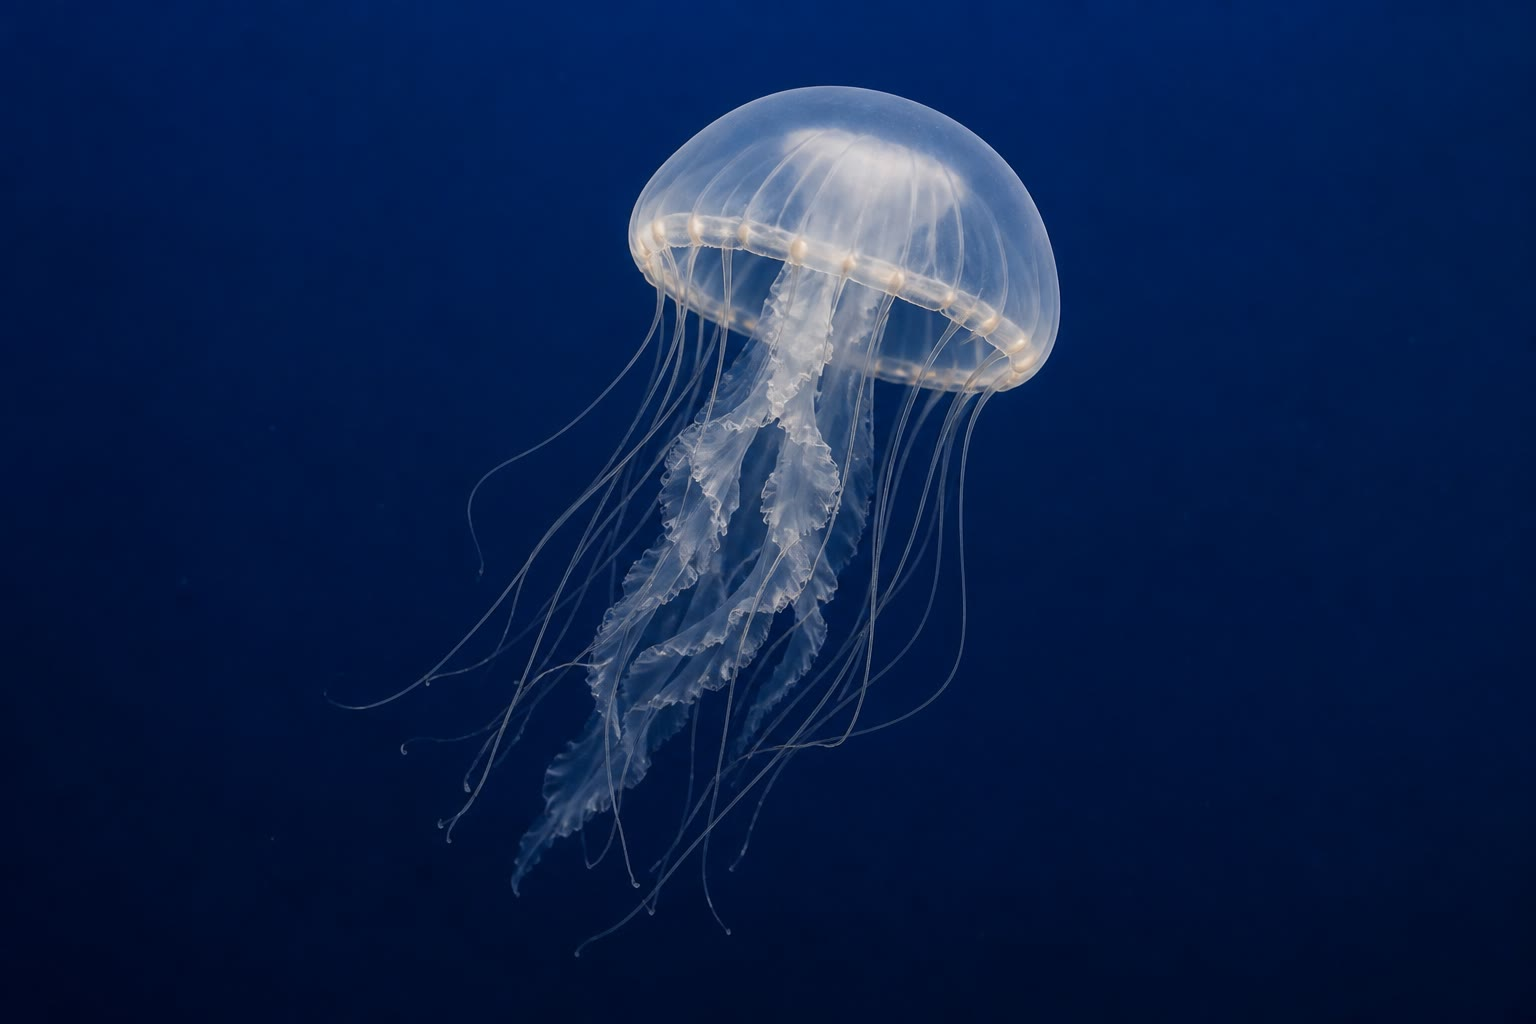
\includegraphics[width=0.46\linewidth]{images/book5/ai/b5-17-jellyfish.jpg}\hspace{0.04\linewidth}
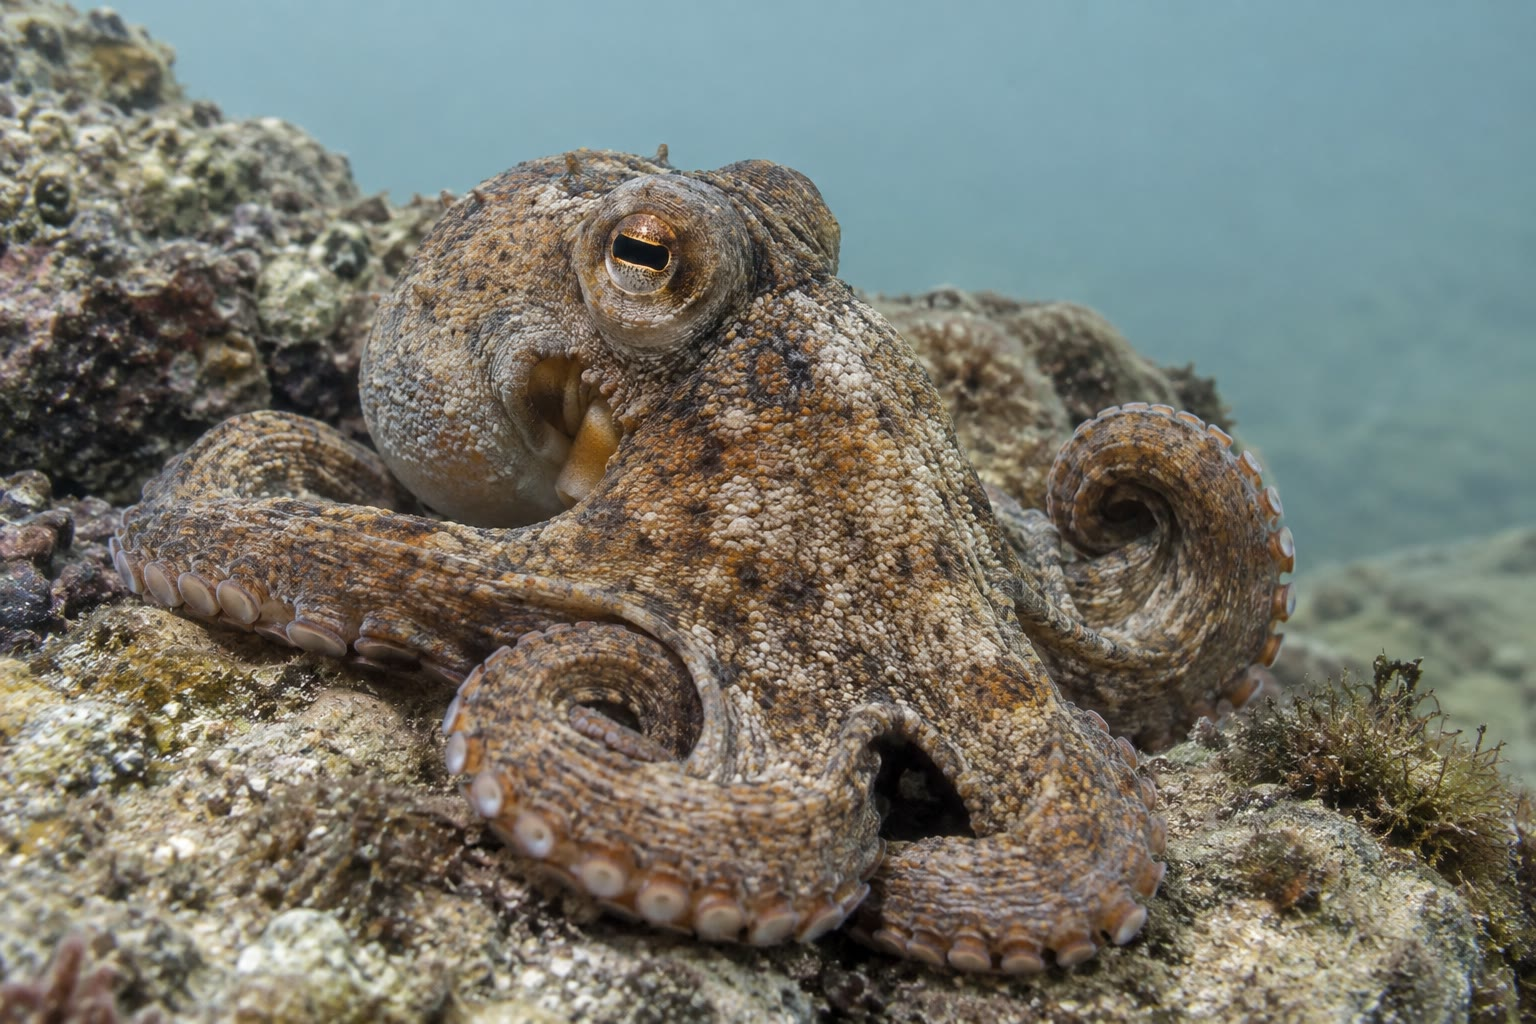
\includegraphics[width=0.46\linewidth]{images/book5/ai/b5-17-octopus.jpg}

{\small Twee manieren om neuronen te ordenen. Links: een kwal, wier
\omterm{def:b3:nervous-systems:comparative}{zenuwnet} en randringen het zwemmen zonder brein coördineren. Rechts:
een octopus, met een half miljard neuronen, de meeste daarvan in de
armen, en het grootste brein van alle ongewervelden.}
\end{omfigure}

\begin{remark}[Waar een zenuwstelsel voor dient]\label{rem:b3:nervous-systems:for}
Planten, schimmels en sponzen hebben er geen; een dier dat zich
beweegt heeft er een nodig, en de uitwerking van zenuwstelsels volgt de
eisen van beweging, van waarnemen op afstand en van voorspellen wat er
daarna gebeurt. De \omterm{thm:b3:nervous-systems:cable}{kabelvergelijking} legt de natuurkunde vast --- hoe
ver en hoe snel een signaal loopt bij een gegeven diameter en isolatie;
de energiebegroting legt de economie vast; en binnen die grenzen
brengen dezelfde neuronen, geordend als netten, ganglia of een schors,
de pulsslag van een kwal, de camouflage van een octopus of deze zin
voort. De volgende twee hoofdstukken nemen het invoereinde en de
opslag: hoe de zintuigen de wereld in pulsen omzetten, en hoe synapsen
veranderen zodat de wereld, eenmaal ontmoet, wordt onthouden.
\end{remark}

\section{Opgaven}

\begin{exercise}[$\star$]\label{exo:b3:nervous-systems:1}
Noem de vier soorten \omterm{def:b3:nervous-systems:cells}{glia} en van elk één functie, en zeg welke twee
\omterm{def:b3:nervous-systems:cells}{myeline} maken en waar.
\end{exercise}

\begin{exercise}[$\star$]\label{exo:b3:nervous-systems:2}
Wat maakte de kleuring van Golgi mogelijk, wat besloot Cajal eruit, en
wat besloot Golgi? Wie had gelijk, en hoe is het beslecht?
\end{exercise}

\begin{exercise}[$\star$]\label{exo:b3:nervous-systems:3}
Beschrijf de \omterm{def:b3:nervous-systems:circuits}{reflexboog} van de kniepeesreflex en leg uit waarom die
maar \qty{30}{ms} kost terwijl een bewuste trap tien maal zo lang duurt.
\end{exercise}

\begin{exercise}[$\star$]\label{exo:b3:nervous-systems:4}
Noem de sympathische en parasympathische effecten op het hart, de
pupil, de darm en de luchtwegen, en de overdrachtsstof die elk deel bij
het doelorgaan gebruikt.
\end{exercise}

\begin{exercise}[$\star\star$]\label{exo:b3:nervous-systems:5}
Bereken de \omterm{thm:b3:nervous-systems:cable}{lengteconstante} van een axon van \qty{1}{\micro m} met $R_{m}
= \qty{1e4}{\ohm.cm^2}$ en $R_{i} = \qty{100}{\ohm.cm}$, en het deel
van een signaal dat na \qty{2}{mm} over is. Welke diameter zou
$\lambda$ verdubbelen?
\end{exercise}

\begin{exercise}[$\star\star$]\label{exo:b3:nervous-systems:6}
Een sensorisch axon van \qty{12}{\micro m} loopt \qty{1.2}{m} van de
teen naar het merg, en een motorisch axon van \qty{15}{\micro m} loopt
terug. Schat met \qty{6}{m/s} per micrometer en \qty{0.5}{ms} per
synaps de kleinste latentie van een spinale terugtrekreflex met één
\omterm{def:b3:nervous-systems:cells}{interneuron}. Hoe lang zou het duren met ongemyeliniseerde axonen van
dezelfde diameter bij $v = 1.1\sqrt{d}$?
\end{exercise}

\begin{exercise}[$\star\star$]\label{exo:b3:nervous-systems:7}
Schat met de begroting van het brein uit
\cref{prop:b3:nervous-systems:barrier-budget} hoeveel ATP een neuron
per seconde kan uitgeven, en, als een puls met zijn synapsen
$2\times 10^{9}$ ATP kost, het gemiddelde vuurtempo dat de begroting
toelaat. Wat voorspelt dat over de codering?
\end{exercise}

\begin{exercise}[$\star\star$]\label{exo:b3:nervous-systems:8}
Leg uit waarom een halfcentrumoscillator vermoeidheid (of een ander
traag proces) nodig heeft om te oscilleren, en wat er zou gebeuren met
twee elkaar remmende neuronen die nooit moe worden.
\end{exercise}

\begin{exercise}[$\star\star$]\label{exo:b3:nervous-systems:9}
De bloed--hersenbarrière sluit dopamine, het product van L-dopa, buiten
maar laat L-dopa toe. Leg uit hoe dat bij de ziekte van Parkinson wordt
benut en waarom antilichamen tegen hersen-eiwitten moeilijk zijn af te
leveren.
\end{exercise}

\begin{exercise}[$\star\star\star$]\label{exo:b3:nervous-systems:10}
Leid de tijdsafhankelijke vorm van de \omterm{thm:b3:nervous-systems:cable}{kabelvergelijking} af,
$\lambda^{2}\,\partial^{2}
V/\partial x^{2} = \tau\,\partial V/\partial t + V$, door de
capacitieve stroom bij de membraanstroom op te tellen, en laat zien dat
de stationaire oplossing van de stelling eruit volgt. (Geef de vorm;
oplossen is niet nodig.) Waarom is de verhouding $\lambda/\tau$ een
snelheid?
\end{exercise}

\begin{exercise}[$\star\star\star$]\label{exo:b3:nervous-systems:11}
Het reuzenaxon van een inktvis van \qty{500}{\micro m} geleidt met
\qty{25}{m/s}. Welke diameter van een ongemyeliniseerd axon zou met
$v \propto \sqrt{d}$ nodig zijn voor \qty{100}{m/s}? Bereken de
doorsnede en vergelijk met het gemyeliniseerde axon van
\qty{20}{\micro m} dat die snelheid haalt. Wat betekent dat voor het
aantal snelle vezels dat een zenuw kan dragen, en voor de evolutie van
\omterm{def:b3:nervous-systems:cells}{myeline}?
\end{exercise}

\begin{exercise}[$\star\star\star$]\label{exo:b3:nervous-systems:12}
De hersenmassa schaalt bij zoogdieren als $M_{\text{body}}^{0.75}$. Een
muis van \qty{30}{g} heeft een brein van \qty{0.4}{g}. Voorspel de
hersenmassa van een zoogdier van \qty{70}{kg} op de lijn, vergelijk met
de menselijke \qty{1350}{g}, en bespreek waarom het aantal neuronen in
de schors een betere maat voor het denkvermogen is dan de hersenmassa.
\end{exercise}

\section{Vraagstuk: een lichaam bedraden}

\begin{problem}[{Weekendvraagstuk --- de bedrading van een lichaam
doorgerekend in lengteconstanten, milliseconden en watt: de
kabelgetallen van een dendriet en twee axonen, de latentie van een
reflex van teen naar merg en terug, de energie die het brein per puls
kan betalen, en de schaling van breinen bij verschillende dieren,
eindigend bij de lengteconstante, de reflexlatentie en het gemiddelde
vuurtempo dat een brein kan bekostigen}]
\label{pb:b3:nervous-systems:1}
Gegevens: $R_{m} = \qty{2e4}{\ohm.cm^2}$, $R_{i} = \qty{100}{\ohm.cm}$,
$C_{m} = \qty{1}{\micro F/cm^2}$. Gemyeliniseerde snelheid \qty{6}{m/s}
per micrometer; ongemyeliniseerd $v = 1.1\sqrt{d}$ m/s met $d$ in
micrometer; synaptische vertraging \qty{0.5}{ms}. Brein: \qty{20}{W},
$8.6\times 10^{10}$ neuronen, $10^{14}$ synapsen, ATP \qty{50}{kJ/mol};
een puls kost $4\times 10^{8}$ ATP en elke synaptische overdracht
$2\times 10^{4}$ ATP; een neuron heeft \num{7000} synapsen. Schaling:
$M_{\text{brain}} = a\,M_{\text{body}}^{0.75}$ met een muis van
\qty{30}{g} die een brein van \qty{0.4}{g} heeft.

\medskip
\noindent\textbf{Deel I --- Kabels.}
\begin{enumerate}
  \item Bereken $\lambda$ voor dendrieten van \qty{1}{\micro m} en
        \qty{4}{\micro m}, en $\tau$.
  \item Een synaps op \qty{300}{\micro m} van het soma op de dendriet
        van \qty{1}{\micro m} brengt plaatselijk \qty{5}{mV} voort. Wat
        komt er bij het soma aan? En op de dendriet van
        \qty{4}{\micro m}?
  \item Leg uit waarom een neuron zijn invoeren kan wegen naar de
        plaats waar zij op de boom terechtkomen, en waarom invoeren
        binnen ongeveer $\tau$ moeten aankomen om op te tellen.
  \item Bereken de snelheid van een gemyeliniseerd axon van
        \qty{10}{\micro m} en van een ongemyeliniseerd axon van
        dezelfde diameter. Welke diameter van een ongemyeliniseerd axon
        zou het gemyeliniseerde evenaren?
  \item Doorsneden van het axon van \qty{10}{\micro m} en van het
        ongemyeliniseerde equivalent. Hoeveel gemyeliniseerde axonen
        passen er in de ruimte van één gelijkwaardig ongemyeliniseerd
        axon?
  \item Een demyeliniserende ziekte haalt over \qty{2}{cm} de \omterm{def:b3:nervous-systems:cells}{myeline}
        van een axon van \qty{10}{\micro m} weg. Schat de extra
        vertraging over dat stuk als het als een ongemyeliniseerd axon
        van die diameter geleidt, en zeg waarom de geleiding geheel kan
        uitvallen.
\end{enumerate}

\medskip
\noindent\textbf{Deel II --- Latenties.}
\begin{enumerate}[resume]
  \item Een teen raakt een heet oppervlak. Het sensorische axon
        (\qty{10}{\micro m}, \qty{1.2}{m}) bereikt het merg, één
        \omterm{def:b3:nervous-systems:cells}{interneuron}, en een motorisch axon (\qty{15}{\micro m},
        \qty{1.1}{m}) keert terug naar het been. Kleinste latentie van
        het terugtrekken?
  \item Het signaal loopt ook \qty{0.6}{m} omhoog langs een axon van
        \qty{10}{\micro m} naar het brein en door nog twee synapsen
        voordat pijn wordt gevoeld. Wanneer wordt de pijn gevoeld ten
        opzichte van het terugtrekken?
  \item Een pijnvezel is ongemyeliniseerd, \qty{1}{\micro m}. Hoe lang
        doet haar signaal over de \qty{1.8}{m} naar het brein? Verklaar
        de twee fasen van de pijn van een gestoten teen.
  \item Het been van een giraf is \qty{2}{m} langer. Bereken de
        reflexlatentie opnieuw en bespreek de problemen van de grootte.
  \item De kniepeesreflex is monosynaptisch, \qty{30}{ms} bij een
        volwassene. Verantwoord de \qty{30}{ms} met \qty{0.8}{m} heen
        en terug bij \qty{80}{m/s}, één synaps en een neuromusculaire
        overgang (\qty{1}{ms}), en \qty{5}{ms} voor de spier om kracht
        op te bouwen.
  \item De axonen van een pasgeborene zijn ongemyeliniseerd. Leg uit
        waarom zijn reflexen traag en zijn bewegingen ongecoördineerd
        zijn, en wat de myelinisatie in de eerste twee jaar verandert.
\end{enumerate}

\medskip
\noindent\textbf{Deel III --- De begroting.}
\begin{enumerate}[resume]
  \item Reken \qty{20}{W} om in ATP per seconde, en in ATP per neuron
        per seconde.
  \item Een neuron vuurt één puls: die kost zelf $4\times 10^{8}$ ATP
        en stuurt \num{7000} synapsen aan van elk $2\times 10^{4}$.
        Totale kosten van één puls met zijn gevolgen?
  \item Welk gemiddeld vuurtempo houdt de begroting vol als zij geheel
        aan pulsen opgaat? En als de helft naar rustkosten gaat?
  \item Neuronen van de schors vuren gemiddeld met ongeveer
        \qty{1}{Hz}. Welk deel van de begroting is dat, en wat betekent
        het voor de manier waarop informatie wordt gecodeerd?
  \item Hoeveel watt zou een brein nodig hebben dat elk neuron met
        \qty{50}{Hz} liet vuren? Vergelijk met de \qty{100}{W} van het
        hele lichaam.
  \item Glucose bereikt het brein met \qty{5}{g/h}. Hoeveel watt is dat
        (\qty{16}{kJ/g})? Is dat genoeg, en wat gebeurt er binnen
        seconden met het bewustzijn als de toevoer uitvalt?
\end{enumerate}

\medskip
\noindent\textbf{Deel IV --- Schaling.}
\begin{enumerate}[resume]
  \item Bepaal $a$ uit de muis en voorspel daarna de hersenmassa van
        een zoogdier van \qty{70}{kg} en van een olifant van
        \qty{5000}{kg} op de lijn.
  \item Werkelijke waarden: mens \qty{1350}{g}, olifant \qty{4800}{g}.
        Bereken voor elke soort de verhouding tot de voorspelling (het
        encefalisatiequotiënt).
  \item Het brein van de olifant heeft $2.6\times 10^{11}$ neuronen
        maar $5.6\times 10^{9}$ in de schors; dat van de mens
        $8.6\times 10^{10}$ en $1.6\times 10^{10}$. Waar zitten de
        neuronen van de olifant, en wat zegt dat over wat de schors
        doet?
  \item Het volume van een neuron groeit met de lengte van zijn axon,
        dus hebben grotere breinen grotere, ijler verspreide neuronen.
        Leg uit waarom een verdubbeling van de hersenmassa het aantal
        neuronen niet verdubbelt, en waarom primaten, wier neuronen
        klein blijven terwijl het brein groeit, meer neuronen per gram
        winnen dan knaagdieren.
  \item Een octopus heeft $5\times 10^{8}$ neuronen, twee derde daarvan
        in zijn armen. Stel voor wat een arm zonder het brein wel en
        niet kan, en één experiment om dat te toetsen.
  \item De rondworm \emph{C.~elegans} heeft $302$ neuronen en in totaal
        ongeveer \num{7000} synapsen, elk in kaart gebracht. Vergelijk
        zijn synapsen per neuron met het menselijke getal, en zeg wat
        een volledig bedradingsschema ons wel en niet over gedrag kan
        vertellen.
  \item Vat samen: de \omterm{thm:b3:nervous-systems:cable}{lengteconstante} van de dendriet van
        \qty{1}{\micro m} (vraag~1), de latentie van de terugtrekreflex
        (vraag~7), en het gemiddelde vuurtempo dat de begroting van het
        brein toelaat als de helft van de energie naar pulsen gaat
        (vraag~15).
\end{enumerate}
\end{problem}
